\begin{pastexam}[label={px:ust-108-ee-ds-05}]{臺聯大電機類 108 學年度 第 5 題}
（問答）

(20\%)Please use recursion to flip(left-right) a binary tree.

ex:
\begin{center}
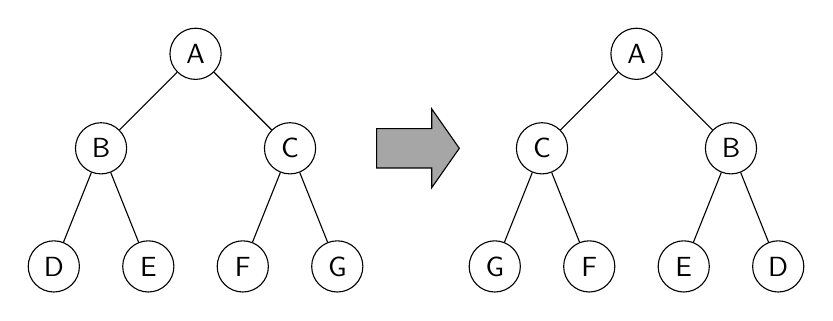
\begin{tikzpicture}[v/.style={circle,draw,inner sep=1pt,minimum size=6.5mm,font=\sffamily}]
\node[v] (LA) at (1.80,0.00) {A};
\node[v] (LB) at (0.60,-1.20) {B};
\node[v] (LC) at (3.00,-1.20) {C};
\node[v] (LD) at (0.00,-2.70) {D};
\node[v] (LE) at (1.20,-2.70) {E};
\node[v] (LF) at (2.40,-2.70) {F};
\node[v] (LG) at (3.60,-2.70) {G};
\draw (LA) -- (LB);
\draw (LA) -- (LC);
\draw (LB) -- (LD);
\draw (LB) -- (LE);
\draw (LC) -- (LF);
\draw (LC) -- (LG);
\node[v] (RA) at (7.40,0.00) {A};
\node[v] (RC) at (6.20,-1.20) {C};
\node[v] (RB) at (8.60,-1.20) {B};
\node[v] (RG) at (5.60,-2.70) {G};
\node[v] (RF) at (6.80,-2.70) {F};
\node[v] (RE) at (8.00,-2.70) {E};
\node[v] (RD) at (9.20,-2.70) {D};
\draw (RA) -- (RC);
\draw (RA) -- (RB);
\draw (RC) -- (RG);
\draw (RC) -- (RF);
\draw (RB) -- (RE);
\draw (RB) -- (RD);
\filldraw[fill=gray!70] (4.10,-0.95) -- (4.80,-0.95) -- (4.80,-0.70) -- (5.15,-1.20) -- (4.80,-1.70) -- (4.80,-1.45) -- (4.10,-1.45) -- cycle;
\end{tikzpicture}
\end{center}
\end{pastexam}

\begin{pastsoln}
左右翻轉（mirror）就是對\textbf{每一個}節點，把它的左子樹和右子樹對調。 遞迴的想法：一棵樹翻好，
等於根的兩棵子樹各自翻好、再把兩棵對調。 空樹不用做事，就是遞迴的終點。

\begin{pseudo}[unbreakable]{把二元樹左右翻轉}
\Procedure{Mirror}{$t$}
    \If{$t = \NIL$}
        \State \Return
    \EndIf
    \State 交換 $t.\mathit{left}$ 和 $t.\mathit{right}$
    \State \Call{Mirror}{$t.\mathit{left}$}
    \State \Call{Mirror}{$t.\mathit{right}$}
\EndProcedure
\end{pseudo}

C 程式（節點有 \texttt{left}、\texttt{right} 兩個指標）：
\begin{minted}[fontsize=\small]{c}
struct TNode {
    char key;
    struct TNode *left, *right;
};

void mirror(struct TNode *t)
{
    struct TNode *tmp;
    if (t == NULL)
        return;
    tmp = t->left;              /* 對調左右子樹 */
    t->left = t->right;
    t->right = tmp;
    mirror(t->left);            /* 兩棵子樹各自翻 */
    mirror(t->right);
}
\end{minted}

\textbf{正確性。} 對樹的節點數 $n$ 做強歸納。 $n = 0$ 是空樹，直接回傳，空樹翻過來還是空樹。
$n \ge 1$ 時，根的左子樹 $L$、右子樹 $R$ 的節點數都小於 $n$。 交換之後根的左邊是 $R$、右邊是 $L$，
再由歸納假設，兩次遞迴呼叫分別把它們翻成 $R$、$L$ 的鏡像。 「左邊是 $R$ 的鏡像、右邊是 $L$ 的
鏡像」正是原樹的鏡像。 先遞迴再交換（後序）也對，先交換再遞迴（前序）就像上面那樣寫，兩種都行；
但不能寫成中序（遞迴左、交換、遞迴右）：交換後的「右」其實是原本的左子樹，原本的左子樹會被翻兩次（等於沒翻），原本的右子樹一次都沒翻。

\textbf{用題目的例子追蹤。} 原樹前序 $A\,B\,D\,E\,C\,F\,G$。
\begin{itemize}
\item \proc{Mirror}$(A)$：交換後 $A$ 的左是 $C$、右是 $B$。
\item \proc{Mirror}$(C)$：交換後 $C$ 的左是 $G$、右是 $F$；$G$、$F$ 是葉，兩邊都是 \NIL，交換不變。
\item \proc{Mirror}$(B)$：交換後 $B$ 的左是 $E$、右是 $D$。
\end{itemize}
結果的前序是 $A\,C\,G\,F\,B\,E\,D$，中序是 $G\,C\,F\,A\,E\,B\,D$（原樹中序 $D\,B\,E\,A\,F\,C\,G$ 的
倒過來），和題目右邊的圖一樣。

\textbf{複雜度。} 每個節點做一次常數時間的交換，\NIL 指標有 $n + 1$ 個，每個也被呼叫一次，
總共 $2n + 1$ 次呼叫，$\Theta(n)$ 時間。 遞迴深度是樹高 $h$，額外空間 $\Theta(h)$，最壞（鏈狀）
$\Theta(n)$。
\end{pastsoln}
